% !TEX TS-program = pdflatexmk

% autor : Lalaso2000
% このテンプレートは配布用で改変可です。
% 作者もこのテンプレのまま使っていません(文字サイズ等に手を加えている)
% 何か問題があればgithubのissueまで

% 以下はC言語で言う所の#include
% 環境によっては必要なパッケージが無いので適宜DLしてください

\documentclass[autodetect-engine,dvipdfmx-if-dvi,ja=standard]{bxjsarticle}
\usepackage{listings,jlisting,ascmac,EMfbox,moreverb,setspace,jquote}
\usepackage{here}
\usepackage{amsmath}
\def\lstlistingname{ソースコード}
\usepackage[at]{easylist}
\usepackage[dvipdfmx]{graphicx}
\usepackage{wrapfig}
\usepackage{eqnarray, array}
\usepackage{url, hyperref}
\usepackage{cite}
\usepackage[dvipdfmx]{graphicx,color}
\usepackage{grffile}
\usepackage{pxjahyper}
\usepackage{framed}
\usepackage{caption}
\captionsetup[figure]{font=sf}
\captionsetup[table]{font=sf}
\usepackage[subrefformat=parens]{subcaption}
\usepackage{multirow}
\usepackage{siunitx}
\usepackage{tabularx}
\usepackage{titlesec}


\resettagform
\newcolumntype{Y}{>{\centering\arraybackslash}X} %中央揃え
\newcolumntype{Z}{>{\raggedleft\arraybackslash}X} %右揃え


\hypersetup{% hyperrefオプションリスト
    setpagesize=false,
    bookmarksnumbered=true,%
    bookmarksopen=true,%
    colorlinks=true,%
    citecolor=black,
    linkcolor=black,
    urlcolor=blue,
}


\lstset{%
    language={python},
    frame={single},
    basicstyle={},%
    identifierstyle={},%
    commentstyle={},%
    keywordstyle={\bfseries},%
    ndkeywordstyle={},%
    stringstyle={\ttfamily},
    breaklines=true,
    columns=[l]{fullflexible},%
    numbers=left,%
    xrightmargin=0zw,%
    xleftmargin=3zw,%
    numberstyle={\scriptsize},%
    stepnumber=1,
    numbersep=1zw,%
    lineskip=-0.5ex%
}

\newcommand{\titlename}[2]{
    \underline{
        \textit{No.}
        \parbox[c][8pt][c]{1.5cm}{
            \begin{center}
                #1
            \end{center}
        }
    }
    ~
    \underline{
        \parbox[c][8pt][c]{3.5cm}{
            \begin{center}
                #2
            \end{center}
        }
    }
}

\newcommand{\titledate}[3]{
    \underline{
        \parbox[c][8pt][c]{1.5cm}{
            \begin{center}
                #1
            \end{center}
        }
        年
        \parbox[c][8pt][c]{1.5cm}{
            \begin{center}
                #2
            \end{center}
        }
        月
        \parbox[c][8pt][c]{1.5cm}{
            \begin{center}
                #3
            \end{center}
        }
        日
    }
}

\newcommand{\tool}[3]{
    \parbox[c][0pt][c]{4.0cm}{#1}
    #2~~~~#3
}

\newcommand{\web}[3]{
    #1
    ~~~~~
    (#2閲覧) \\
    \url{#3}
}

\renewcommand{\labelenumi}{(\arabic{enumi})}

\makeatletter
\newcommand{\figcaption}[1]{\def\@captype{figure}\caption{#1}}
\newcommand{\tblcaption}[1]{\def\@captype{table}\caption{#1}}
\makeatother

\setcounter{page}{-1}



%================================================================
%文章スタート
%================================================================
\begin{document}

%表紙
\thispagestyle{empty}
\rightline{
    \fontsize{8pt}{0pt} \selectfont
    岐~~阜~~工~~業~~高~~等~~専~~門~~学~~校
}
\vspace{1cm}
\begin{center}
    \fontsize{30pt}{0pt} \selectfont
    電~気~情~報~工~学~実~験~報~告~書
\end{center}
\vspace{1.4cm}
\begin{center}
    \underline{
        \fontsize{14pt}{0pt} \selectfont
        実~~験~~番~~号~~~~~~~~~~~
        \fontsize{18pt}{0pt} \selectfont
        %実験番号!!=====================================================================================
        0
        %記入し忘れ注意!=================================================================================
        \fontsize{14pt}{0pt} \selectfont
        ~~~~~~~~~~~
    }
\end{center}
\vspace{0.4cm}
\begin{table}[h]
    \begin{center}
        \begin{tabular}{| c | l |} \hline
            \parbox[c][1.5cm][c]{0cm}{}
            ~~~~実~~験~~題~~目~~~~ &
            \parbox[c][1.5cm][c]{12cm}{
                \fontsize{14pt}{0pt} \selectfont
                %実験題目!!=============================================================================
                レポートの書き方
                %記入し忘れ注意!==========================================================================
            }
            \\ \hline
        \end{tabular}
    \end{center}
\end{table}

\begin{table}[h]
    \begin{center}
        \begin{tabularx}{13cm}{|c|Y|} \hline
            \multirow{4}{*}{
                報~告~書~提~出~者
            }
            & ~ \\
            & \underline{
                ~~~~~~
                %班番号===================================================================================
                0
                %=========================================================================================
                ~~~~~~班
            } \\
            & ~ \\
            & \underline{
                学年~~~
                %学年=====================================================================================
                4
                %=========================================================================================
                ~~~
            }
            ~
            %名列番号と名前===============================================================================
            \titlename{00}{Lalaso2000}
            %=============================================================================================
            \\[5pt]
            \hline

            \multirow{7}{*}{
                共~測~者~氏~名
            }
            & ~ \\
            %班のメンバーの名列と名前
            & \titlename{xx}{山田太郎}
            \\[5pt]
            & \titlename{}{}
            \\[5pt]
            & \titlename{}{}
            \\[5pt]
            & \titlename{}{}
            \\[5pt]
            & \titlename{}{}
            \\[5pt]
            & \titlename{}{}
            %============================================================================================
            \\[5pt]
            \hline
        \end{tabularx}
    \end{center}
\end{table}

\begin{table}[h]
    \begin{minipage}{0.7\hsize}
        \begin{center}
            \begin{tabularx}{10cm}{ Y  c }
                \underline{
                    \parbox[c][8pt][c]{2.5cm}{
                        \begin{center}
                            実~験~実~施~日
                        \end{center}
                    }
                }
                %実験実施日==============================================================================
                & \titledate{29}{9}{29} \\[8pt]
                & \titledate{}{}{} \\[8pt]
                & \titledate{}{}{} \\[8pt]
                %========================================================================================
                \underline{
                    \parbox[c][8pt][c]{2.5cm}{
                        \begin{center}
                            報~告~書~提~出~日
                        \end{center}
                    }
                }  &
                %報告書提出日===========================================================================
                \titledate{29}{10}{1} \\[15pt]
                %=======================================================================================
                & \fontsize{7pt}{0pt} \selectfont
                電 気 情 報 工 学 科 \\
            \end{tabularx}
        \end{center}
    \end{minipage}
    \begin{minipage}{0.3\hsize}
        \begin{center}
            \captionsetup{labelformat=empty,labelsep=none}
            \caption{採点}
            \begingroup
                \renewcommand{\arraystretch}{1.2}
                \begin{tabularx}{3cm}{| c | Y |} \hline
                    {\gt 体裁} & \\ \hline
                    {\gt 原理} & \\ \hline
                    {\gt 内容} & \\ \hline
                    {\gt 考察} & \\ \hline \hline
                    {\gt 合計点} & \\ \hline
                \end{tabularx}
            \endgroup
        \end{center}
    \end{minipage}
\end{table}

\newpage

\newgeometry{top=25.4mm, bottom=25.4mm, left=19.05mm, right=19.05mm}
\thispagestyle{empty}
○教員からのコメント


\newpage
\setcounter{table}{0}



%ココから本文============================================================================================
\section{実験年月日}
平成29年9月29日  天候:晴れ  気温:20℃  湿度:33.4%


\section{実験の目的}
実験レポートをより良くするため、書き方を理解する。



\section{実験の理論}
\subsection{理論の書き方}
3年までの実験書には、詳しい理論が書いてあったため、
それを写す感じでも大丈夫であったが、
4年以降の実験書は書いていないことが多くなるため、
自力で調査する必要がある。
また、実験書で調べるべきことが指定されている場合もある。

理論をしっかり調べることによって考察や検討課題は圧倒的に楽になるため、
できるだけたくさん調べてまとめると良い。


\subsubsection{参考文献}
% 太字と斜体
\textbf{参考文献}(\textit{Bibliography})とは、
書物・論文などにまとめるうえで、参考とする書物・文書のことである。
\cite{辞書}
今日のレポートでは、書物の他、Webページになることもある。

\textbf{たった今示した通り、文章の途中で引用した箇所の後ろに括弧を付けて
番号をうち、レポートの末尾に参考文献の一覧を示すのが正しい書き方である。}

参考文献を示さずに引用を行うとコピー&ペーストとなり、
重大な問題となるので注意が必要である。


\subsubsection{図・表の扱い}

% wrapfigure(回り込みで図を入れる)
% wraptableもある
% 3cmとなっているところは、画像の大きさに合わせて変える
% よくめり込んだり他のモノに弊害を及ぼす時があるので、vspaceの数字をいじって調整する
\begin{wrapfigure}{r}{3cm}
    % 縦方向の余白、負だと上にずれる。
    \vspace{-2\baselineskip}
    \centering
    % 画像ファイル名はtexファイルのあるディレクトリからの相対パスで書く
    
\includegraphics[width=3cm]{データ/単位を落とす人.png}
    % captionは図のタイトル
    \caption{単位を落としちゃった人}
    % labelは文章中から参照する時の目印
    \label{img/単位}
    \vspace{-1\baselineskip}
\end{wrapfigure}

これは3年時と変わらない。
図番号、表番号を連番にし、文章中で適切に引用するべきである。
図・表のタイトルは、その図や表が何を示しているかが
ひと目で分かるようにするべきである。

関係ないが、レポートをしっかり書かないと図\ref{img/単位}の
ように単位を落としかねない。
% こんな感じで、図○の数字は\ref{(labelで指定した文字列)}を使うと自動で入る
実験はスーパー必修であり、単位を落とすと進級出来なくなるので
注意が必要である。

また、表はWordの表を使うよりも、Excelを用いて表を作り、
画像として保存後、Wordに貼り付ける方法を使うと、
見た目がきれいになりやすい。
グラフはpythonを使うという手もある。
(ソースコード\ref{sc/graph}、図\ref{img/graph}参照)

% ソースコード挿入例
\lstinputlisting[caption=グラフプログラム例, label=sc/graph, basicstyle=\ttfamily]{データ/graph.py}


% 画像挿入(図)
% [h]のhはhereのh。これが書かれた場所(のできるだけ近く)に図が表示される
% h以外にt(top=ページの上の方に表示)、
% b(bottom=ページの下の方)、
% p(page=画像だけのページを作る)
% H(HERE=画像が入り切らなくても絶対これが書かれた位置)等がある

% 余談:LaTeXインストール時に"pdfcrop"っていうのがmacにはついてきた
% 図として挿入するpdfファイルの余白を消してLaTeXで使いやすくしてくれる
\begin{figure}[h]
	\centering
	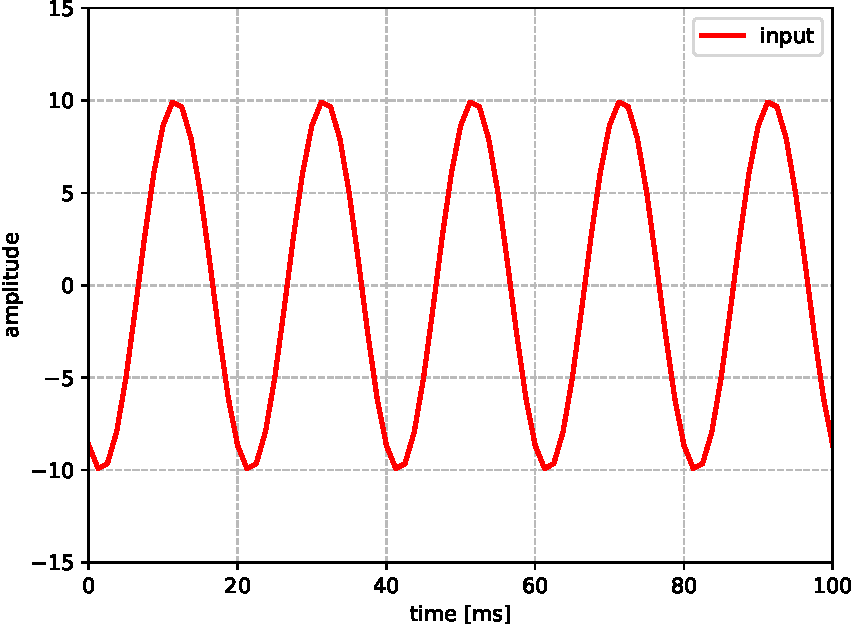
\includegraphics[width=14cm]{データ/graph-crop.pdf}
	\caption{グラフ例}
    \label{img/graph}
    \vspace{-1\baselineskip}
\end{figure}


\section{使用器具}
% 表挿入例
% 基本的にはfigureと同じ
\begin{table}[h]
	\vspace{-0.5\baselineskip}
    \centering
    % 表の説明(caption)は表の上
    \caption{使用器具一覧}
    \label{tb/使用器具}
	
\includegraphics[width=17cm]{データ/使用器具-crop.pdf}
\end{table}



\section{実験方法}
\subsection{実験方法を書く}
% 番号リストはenumerate、箇条書きはitemize
% easylistと言うパッケージもある(wrapfigureとの相性が悪いが…)
\begin{enumerate}
    \item 実験書を開いた。
    \item 実験書を参考にしながら、実際の実験の手順を思い出した。
    \item やった手順をそのまま書いた。
    \begin{itemize}
        \item 気をつけた点なども一緒に書いた。
        \item 過去形にすることを気をつけた。
    \end{itemize}
\end{enumerate}



\section{結果・考察}
\subsection{結果・考察の書き方}
実際には上のタイトルは実験方法と揃えておくと、書きやすくなる。

レポートを書いたことによって、
4年以降のレポートは実験結果と考察を一緒に書く事が分かった。
これは、このように結果と考察をまとめて書いたほうが、
どの結果に対する考察なのかがわかりやすく、
読みやすいからであると考えられる。

結果は、\textbf{ありのままに起こったこと}であり
測定結果や見た目の変化などを述べるべきである。
一方考察は、\textbf{結果から考えられること}であり、
結果を受けてさらに想像したことを述べるべきである。
上の文を例に取れば、「レポートを書いたことによって…分かった」
は結果であり、「これは…考えられる」は考察である。

また、表やグラフを活用するべきであることも分かった。
これらはExcelやpython等で作成し、画像として保存してから
貼り付けると、見た目が崩れないため良いと思われる。



\section{検討課題}
\subsection{検討課題について}
検討課題は与えられたものを書いていけばよいが、
まれに考察に含んでしまったほうが書きやすいものもある。
そういう場合は考察に含めてOKである。

\subsection{Word以外のレポートの作り方}
このテンプレはWordで作成したものではなく、\textbf{LaTeX}という
ものを使用して作成したものである。
LaTeXとは、書籍等の文章を作成するための組版システムであり、
特定のソフトウェアではなく、HTMLのようにコードを書いて、
特定の方法で出力するとレポートが書ける。
\cite{LaTeX}

図表の位置を自動で調整してくれたり、図表番号を自動で管理してくれたり、
見た目(特に数式)もかなり良くなるのでおすすめである。
環境構築や慣れるまでが少し大変(特に図表の扱い)だが、
論文はLaTeXで書くことが多いため、やって損はないと思う。

% 数式の書き方が溢れた
% 数式については
% http://cns-guide.sfc.keio.ac.jp/2001/11/4/1.html
% を参照されたり

\begin{thebibliography}{99}
\bibitem{辞書} \web{Weblio辞書}{2017/09/30}{http://www.weblio.jp/}
\bibitem{LaTeX} \web{LaTeX入門 - TeX Wiki}{2017/09/30}{https://texwiki.texjp.org/?LaTeX\%E5\%85\%A5\%E9\%96\%80}
\end{thebibliography}


\end{document}
